% Options for packages loaded elsewhere
\PassOptionsToPackage{unicode}{hyperref}
\PassOptionsToPackage{hyphens}{url}
\PassOptionsToPackage{dvipsnames,svgnames,x11names}{xcolor}
%
\documentclass[
  letterpaper,
  DIV=11,
  numbers=noendperiod]{scrartcl}

\usepackage{amsmath,amssymb}
\usepackage{iftex}
\ifPDFTeX
  \usepackage[T1]{fontenc}
  \usepackage[utf8]{inputenc}
  \usepackage{textcomp} % provide euro and other symbols
\else % if luatex or xetex
  \usepackage{unicode-math}
  \defaultfontfeatures{Scale=MatchLowercase}
  \defaultfontfeatures[\rmfamily]{Ligatures=TeX,Scale=1}
\fi
\usepackage{lmodern}
\ifPDFTeX\else  
    % xetex/luatex font selection
\fi
% Use upquote if available, for straight quotes in verbatim environments
\IfFileExists{upquote.sty}{\usepackage{upquote}}{}
\IfFileExists{microtype.sty}{% use microtype if available
  \usepackage[]{microtype}
  \UseMicrotypeSet[protrusion]{basicmath} % disable protrusion for tt fonts
}{}
\makeatletter
\@ifundefined{KOMAClassName}{% if non-KOMA class
  \IfFileExists{parskip.sty}{%
    \usepackage{parskip}
  }{% else
    \setlength{\parindent}{0pt}
    \setlength{\parskip}{6pt plus 2pt minus 1pt}}
}{% if KOMA class
  \KOMAoptions{parskip=half}}
\makeatother
\usepackage{xcolor}
\setlength{\emergencystretch}{3em} % prevent overfull lines
\setcounter{secnumdepth}{-\maxdimen} % remove section numbering
% Make \paragraph and \subparagraph free-standing
\ifx\paragraph\undefined\else
  \let\oldparagraph\paragraph
  \renewcommand{\paragraph}[1]{\oldparagraph{#1}\mbox{}}
\fi
\ifx\subparagraph\undefined\else
  \let\oldsubparagraph\subparagraph
  \renewcommand{\subparagraph}[1]{\oldsubparagraph{#1}\mbox{}}
\fi


\providecommand{\tightlist}{%
  \setlength{\itemsep}{0pt}\setlength{\parskip}{0pt}}\usepackage{longtable,booktabs,array}
\usepackage{calc} % for calculating minipage widths
% Correct order of tables after \paragraph or \subparagraph
\usepackage{etoolbox}
\makeatletter
\patchcmd\longtable{\par}{\if@noskipsec\mbox{}\fi\par}{}{}
\makeatother
% Allow footnotes in longtable head/foot
\IfFileExists{footnotehyper.sty}{\usepackage{footnotehyper}}{\usepackage{footnote}}
\makesavenoteenv{longtable}
\usepackage{graphicx}
\makeatletter
\def\maxwidth{\ifdim\Gin@nat@width>\linewidth\linewidth\else\Gin@nat@width\fi}
\def\maxheight{\ifdim\Gin@nat@height>\textheight\textheight\else\Gin@nat@height\fi}
\makeatother
% Scale images if necessary, so that they will not overflow the page
% margins by default, and it is still possible to overwrite the defaults
% using explicit options in \includegraphics[width, height, ...]{}
\setkeys{Gin}{width=\maxwidth,height=\maxheight,keepaspectratio}
% Set default figure placement to htbp
\makeatletter
\def\fps@figure{htbp}
\makeatother

\KOMAoption{captions}{tableheading,figureheading}
\makeatletter
\makeatother
\makeatletter
\makeatother
\makeatletter
\@ifpackageloaded{caption}{}{\usepackage{caption}}
\AtBeginDocument{%
\ifdefined\contentsname
  \renewcommand*\contentsname{Tabla de contenidos}
\else
  \newcommand\contentsname{Tabla de contenidos}
\fi
\ifdefined\listfigurename
  \renewcommand*\listfigurename{Listado de Figuras}
\else
  \newcommand\listfigurename{Listado de Figuras}
\fi
\ifdefined\listtablename
  \renewcommand*\listtablename{Listado de Tablas}
\else
  \newcommand\listtablename{Listado de Tablas}
\fi
\ifdefined\figurename
  \renewcommand*\figurename{Figura}
\else
  \newcommand\figurename{Figura}
\fi
\ifdefined\tablename
  \renewcommand*\tablename{Tabla}
\else
  \newcommand\tablename{Tabla}
\fi
}
\@ifpackageloaded{float}{}{\usepackage{float}}
\floatstyle{ruled}
\@ifundefined{c@chapter}{\newfloat{codelisting}{h}{lop}}{\newfloat{codelisting}{h}{lop}[chapter]}
\floatname{codelisting}{Listado}
\newcommand*\listoflistings{\listof{codelisting}{Listado de Listados}}
\makeatother
\makeatletter
\@ifpackageloaded{caption}{}{\usepackage{caption}}
\@ifpackageloaded{subcaption}{}{\usepackage{subcaption}}
\makeatother
\makeatletter
\@ifpackageloaded{tcolorbox}{}{\usepackage[skins,breakable]{tcolorbox}}
\makeatother
\makeatletter
\@ifundefined{shadecolor}{\definecolor{shadecolor}{rgb}{.97, .97, .97}}
\makeatother
\makeatletter
\makeatother
\makeatletter
\makeatother
\ifLuaTeX
\usepackage[bidi=basic]{babel}
\else
\usepackage[bidi=default]{babel}
\fi
\babelprovide[main,import]{spanish}
% get rid of language-specific shorthands (see #6817):
\let\LanguageShortHands\languageshorthands
\def\languageshorthands#1{}
\ifLuaTeX
  \usepackage{selnolig}  % disable illegal ligatures
\fi
\usepackage[]{biblatex}
\addbibresource{../../../../references.bib}
\IfFileExists{bookmark.sty}{\usepackage{bookmark}}{\usepackage{hyperref}}
\IfFileExists{xurl.sty}{\usepackage{xurl}}{} % add URL line breaks if available
\urlstyle{same} % disable monospaced font for URLs
\hypersetup{
  pdftitle={Introducción a organización industrial},
  pdfauthor={Edison Achalma},
  pdflang={es},
  colorlinks=true,
  linkcolor={blue},
  filecolor={Maroon},
  citecolor={Blue},
  urlcolor={Blue},
  pdfcreator={LaTeX via pandoc}}

\title{Introducción a organización industrial}
\usepackage{etoolbox}
\makeatletter
\providecommand{\subtitle}[1]{% add subtitle to \maketitle
  \apptocmd{\@title}{\par {\large #1 \par}}{}{}
}
\makeatother
\subtitle{Explorando los pilares fundamentales para comprender el
funcionamiento y éxito de la industria moderna}
\author{Edison Achalma}
\date{2023-06-12}

\begin{document}
\maketitle
\ifdefined\Shaded\renewenvironment{Shaded}{\begin{tcolorbox}[frame hidden, interior hidden, borderline west={3pt}{0pt}{shadecolor}, enhanced, breakable, sharp corners, boxrule=0pt]}{\end{tcolorbox}}\fi

\hypertarget{quuxe9-estudiaremos-en-organizaciuxf3n-industrial}{%
\section{¿Qué estudiaremos en organización
industrial?}\label{quuxe9-estudiaremos-en-organizaciuxf3n-industrial}}

Exploraremos una serie de temas fundamentales que nos ayudarán a
comprender la dinámica empresarial y los mercados en los que operan. A
través de un análisis detallado, profundizaremos en los siguientes
aspectos:

\begin{enumerate}
\def\labelenumi{\arabic{enumi}.}
\item
  \textbf{Concentración, poder y competencia económica:} Estudiaremos
  cómo se concentra el poder económico en ciertas empresas y cómo esto
  afecta la competencia en el mercado. Analizaremos casos de monopolios
  y oligopolios, así como las estrategias que utilizan estas empresas
  para mantener su posición dominante.
\item
  \textbf{Diferenciación de producto:} Examinaremos cómo las empresas
  buscan diferenciarse a través de características únicas en sus
  productos o servicios. Analizaremos cómo esta diferenciación afecta la
  demanda y la competencia en el mercado.
\item
  \textbf{Diversificación de productos:} Abordaremos el tema de la
  diversificación empresarial, es decir, cómo las empresas amplían su
  cartera de productos o servicios. Exploraremos los motivos detrás de
  esta estrategia y evaluaremos sus implicaciones para la competencia y
  la rentabilidad de las empresas.
\item
  \textbf{Integración vertical:} Estudiaremos cómo las empresas pueden
  optar por integrarse verticalmente, es decir, controlar distintas
  etapas de la cadena de suministro. Analizaremos los beneficios y
  desafíos de esta estrategia, así como su impacto en la competencia y
  la eficiencia del mercado.
\item
  \textbf{Estructura de mercado en países desarrollados:} Analizaremos
  la estructura de mercado en países con economías avanzadas, explorando
  cómo se organizan las empresas y cuál es el grado de competencia en
  estos mercados. Investigaremos las políticas públicas y regulaciones
  que influyen en la estructura y el comportamiento de las empresas.
\item
  \textbf{Estructura de mercado en países emergentes:} Nos adentraremos
  en el análisis de la estructura de mercado en países con economías en
  desarrollo, examinando las particularidades y los desafíos que
  enfrentan. Estudiaremos cómo se desarrollan los mercados en estas
  naciones y qué factores influyen en su evolución.
\end{enumerate}

\hypertarget{definiciuxf3n-de-organizaciuxf3n-industrial}{%
\section{Definición de Organización
Industrial}\label{definiciuxf3n-de-organizaciuxf3n-industrial}}

La Organización Industrial se centra en el estudio de cómo las empresas
se organizan dentro de los mercados, con el objetivo de analizar y
comprender aspectos como la determinación de precios, cantidades
producidas, costos, poder de mercado y concentración. Es importante
tener en cuenta que estas decisiones y comportamientos empresariales
están condicionados por las políticas públicas y las regulaciones
establecidas, las cuales pueden limitar ciertas acciones y establecer un
marco de actuación para las empresas.

\hypertarget{conceptos-generales}{%
\section{Conceptos Generales}\label{conceptos-generales}}

\hypertarget{poluxedticas-puxfablicas-y-regulaciuxf3n}{%
\subsection{Políticas Públicas y
regulación}\label{poluxedticas-puxfablicas-y-regulaciuxf3n}}

Las políticas públicas y la regulación desempeñan un papel crucial en la
Organización Industrial. Estas intervenciones gubernamentales buscan
corregir fallas de mercado, promover la competencia y proteger los
intereses de los consumidores. Se analizarán los diferentes instrumentos
y mecanismos utilizados para regular y controlar el comportamiento de
las empresas en beneficio de la sociedad.

\hypertarget{recursos-humanos}{%
\subsection{Recursos humanos}\label{recursos-humanos}}

El factor humano es un elemento central en la Organización Industrial.
El estudio de los recursos humanos en las empresas se enfoca en entender
cómo se gestionan y aprovechan los talentos y habilidades de los
empleados, así como en analizar las relaciones laborales y las políticas
de remuneración que impactan en la productividad y competitividad de las
organizaciones.

\hypertarget{factores-de-producciuxf3n}{%
\subsection{Factores de producción}\label{factores-de-producciuxf3n}}

La Organización Industrial también aborda el análisis de los factores de
producción, que son los insumos necesarios para la producción de bienes
y servicios. Se examinan aspectos como la oferta y demanda de los
factores productivos, la tecnología empleada y la asignación eficiente
de los recursos en el proceso productivo.

\hypertarget{el-mercado}{%
\subsection{El mercado}\label{el-mercado}}

El mercado es el escenario donde se desenvuelven las empresas y se lleva
a cabo el intercambio de bienes y servicios. En la Organización
Industrial se analizan las interacciones entre los diferentes agentes
económicos presentes en el mercado, como empresas, consumidores y
proveedores, y se estudia cómo estas interacciones determinan los
precios, la cantidad producida y otros aspectos relevantes para el
funcionamiento de la economía.

\hypertarget{la-economuxeda}{%
\subsection{La economía}\label{la-economuxeda}}

La economía es una disciplina que estudia cómo se asignan los recursos
escasos para satisfacer las necesidades y deseos humanos. Analiza cómo
las personas, las empresas y los gobiernos toman decisiones para
producir, distribuir y consumir bienes y servicios en un entorno de
escasez.

\hypertarget{la-empresa}{%
\subsection{La empresa}\label{la-empresa}}

Una empresa es una organización o entidad que se dedica a la producción
y venta de bienes o servicios con el objetivo de obtener beneficios. Las
empresas pueden ser de distintos tamaños y operar en diferentes sectores
de la economía. Son el motor principal de la actividad económica y
generan empleo y riqueza en las comunidades.

\hypertarget{microeconomuxeda}{%
\subsection{Microeconomía}\label{microeconomuxeda}}

La microeconomía es una rama de la economía que se centra en el estudio
del comportamiento individual de agentes económicos, como consumidores,
empresas y trabajadores, y cómo interactúan en los mercados. Examina
cómo se determinan los precios, la oferta y la demanda, y cómo las
decisiones individuales afectan la asignación de recursos.

\hypertarget{industria}{%
\subsection{Industria}\label{industria}}

La industria se refiere a un conjunto de empresas que producen bienes o
servicios similares. Puede ser un sector específico de la economía, como
la industria automotriz o la industria alimentaria. El análisis de la
industria ayuda a comprender la competencia, la concentración de mercado
y otros factores que influyen en el desempeño de las empresas.

\hypertarget{organizaciuxf3n-industrial}{%
\subsection{Organización Industrial}\label{organizaciuxf3n-industrial}}

La Organización Industrial es una disciplina que se enfoca en el estudio
de cómo se organizan las empresas en los mercados y cómo esto afecta la
estructura de la industria, el comportamiento de las empresas y los
resultados económicos. Examina la relación entre la estructura del
mercado (número de competidores, barreras de entrada, concentración), la
conducta de las empresas (estrategias de precios, publicidad,
diferenciación) y los resultados económicos (eficiencia, poder de
mercado).

\hypertarget{definiciones-sobre-la-organizaciuxf3n-industrial}{%
\section{Definiciones sobre la organización
industrial}\label{definiciones-sobre-la-organizaciuxf3n-industrial}}

La Organización Industrial, como disciplina, ha sido objeto de estudio y
reflexión por parte de destacados expertos en economía. A continuación,
presentaremos tres definiciones clave que nos ayudarán a comprender su
alcance y relevancia:

Según Stigler (1968), la Organización Industrial implica la aplicación
de la teoría microeconómica para analizar el funcionamiento de empresas,
mercados e industrias. En otras palabras, se enfoca en cómo interactúan
y operan estos agentes económicos, considerando aspectos como la
competencia, los precios y los resultados obtenidos.

Tirole (1988), define la economía industrial como el estudio de cómo las
fuerzas del mercado afectan el comportamiento de los actores
involucrados y los resultados que obtienen. Aquí se pone énfasis en
comprender cómo se desarrollan las interacciones en el mercado, cómo
influyen las decisiones de los agentes económicos y qué consecuencias se
derivan de ellas.

Para Scherer y Ross (1998), la economía industrial se ocupa de analizar
cómo las fuerzas del mercado permiten que los planes de los productores
se ajusten a las demandas de los consumidores. También examina cómo la
intervención externa puede afectar este proceso de ajuste y cómo los
resultados obtenidos se comparan con los resultados ideales o esperados.

\begin{quote}
En el desarrollo de la Organización Industrial, también destacan Mason
como Bain quienes realizaron valiosas contribuciones. Mason se enfocó en
la teoría del oligopolio, introduciendo conceptos como la cuota de
mercado y la concentración recíproca. Por su parte, Bain desarrolló el
paradigma de estructura, conducta y resultado (ECR), demostrando la
influencia de la estructura de mercado en la conducta de las empresas y
los resultados económicos. Ambos investigadores analizaron temas como
estrategias de precios, colusión, publicidad, diferenciación de
productos y barreras de entrada. Sus estudios han sido fundamentales
para comprender la dinámica de la competencia y el comportamiento
empresarial en diversas industrias.
\end{quote}

Según el paradigma de estructura, conducta, resultado (ECR) de la
organización industrial desarrollado por Joe S. Bain Jr., los términos
se definen de la siguiente manera:

\textbf{Estructura:} Se refiere a las características y condiciones del
mercado en el que opera una industria. Esto incluye el número de
empresas que existen en el mercado, su tamaño relativo, las barreras de
entrada y salida, la concentración de mercado y la naturaleza de la
competencia.

\textbf{Conducta:} Hace referencia a las acciones y estrategias que las
empresas llevan a cabo en el mercado. Esto implica decisiones
relacionadas con la fijación de precios, la inversión en investigación y
desarrollo, la publicidad y promoción, la diferenciación de productos,
la búsqueda de economías de escala, entre otros factores.

\textbf{Resultado:} Se refiere a los efectos o consecuencias que se
derivan de la estructura y conducta de las empresas en el mercado. Esto
puede incluir el nivel de competencia, los precios de los productos, la
eficiencia económica, la innovación, la calidad de los productos, la
distribución equitativa de recursos, el bienestar del consumidor y la
rentabilidad de las empresas.

\hypertarget{relaciuxf3n-entre-economuxeda-y-organizaciuxf3n-industrial}{%
\section{Relación entre economía y organización
industrial}\label{relaciuxf3n-entre-economuxeda-y-organizaciuxf3n-industrial}}

En el ámbito de la economía y la organización industrial, existe una
estrecha relación que ha evolucionado a lo largo del tiempo. La
economía, como disciplina académica, se ha adaptado a los cambios en las
estructuras de mercado tanto en el sector privado como en el público. Ha
analizado y determinado la forma en que las empresas, las industrias y
los consumidores se comportan en el mercado, así como también ha
cuantificado los niveles de eficiencia y eficacia en sus actividades.

Es importante destacar que la economía no solo se limita a describir y
analizar el funcionamiento de los mercados, sino que también se ha
involucrado en la implementación de políticas y regulaciones que buscan
alinear los intereses públicos y privados. Los reguladores, en este
caso, desempeñan un papel fundamental al intervenir en el mercado para
garantizar que las empresas y los agentes económicos actúen de manera
responsable y en beneficio de la sociedad en su conjunto.

La organización industrial, por su parte, se enmarca dentro de este
contexto económico. Su objetivo es comprender cómo se estructuran las
empresas en los mercados, cómo interactúan y cómo influyen en la
competencia y en los resultados económicos. A través de un análisis
detallado de la estructura de mercado, la conducta de las empresas y los
resultados obtenidos, la organización industrial proporciona
herramientas y conocimientos para entender cómo se organizan y operan
las industrias en un entorno económico determinado.

\hypertarget{estrateguxedas-y-decisiones-estratuxe9gicas}{%
\section{Estrategías y decisiones
estratégicas}\label{estrateguxedas-y-decisiones-estratuxe9gicas}}

\textbf{La importancia de la estrategia:} En el ámbito empresarial, la
estrategia es un documento que establece las acciones y reacciones
necesarias para enfrentar diferentes contingencias y optimizar los
recursos disponibles. Es un plan detallado que guía el rumbo de la
empresa y define cómo interactúa con sus competidores.

\textbf{Decisiones estratégicas y su impacto:} Una decisión se considera
estratégica cuando la acción elegida por un actor económico genera una
reacción en otros actores como empresas, proveedores, compradores y
reguladores. Estas decisiones tienen un impacto significativo en el
entorno empresarial y en la forma en que se desarrollan las relaciones
comerciales.

\textbf{Tipos de decisiones estratégicas:} Las decisiones estratégicas
pueden dividirse en dos categorías:

\begin{itemize}
\item
  Decisiones tácticas: Estas decisiones se centran en acciones a corto
  plazo y están relacionadas con la implementación de la estrategia
  general de la empresa. Implican la asignación de recursos y la
  ejecución de planes para alcanzar objetivos específicos.
\item
  Decisiones con compromisos: Estas decisiones involucran acuerdos y
  compromisos a largo plazo con otros actores económicos. Pueden incluir
  alianzas estratégicas, contratos a largo plazo con proveedores o
  clientes, o incluso decisiones de inversión en nuevas tecnologías o
  mercados.
\end{itemize}

\hypertarget{decisiones-con-compromiso-en-la-organizaciuxf3n-industrial}{%
\subsection{Decisiones con Compromiso en la Organización
Industrial}\label{decisiones-con-compromiso-en-la-organizaciuxf3n-industrial}}

En la dinámica de la organización industrial, existen decisiones que van
más allá de las simples acciones tácticas y tienen un alcance
estratégico a largo plazo. Estas decisiones con compromiso juegan un
papel fundamental en la configuración de la empresa y su relación con el
entorno económico. A continuación, exploraremos algunas de estas
decisiones clave y su impacto en el ámbito empresarial.

\hypertarget{fusiones-y-adquisiciones-expandiendo-el-horizonte}{%
\subsubsection{Fusiones y Adquisiciones: Expandiendo el
horizonte}\label{fusiones-y-adquisiciones-expandiendo-el-horizonte}}

Las fusiones y adquisiciones son decisiones estratégicas que tienen como
objetivo unir fuerzas con otras empresas para lograr sinergias y
aprovechar nuevas oportunidades de mercado. Mediante la integración de
recursos y capacidades, las empresas pueden aumentar su competitividad,
acceder a nuevos segmentos de clientes y ampliar su presencia
geográfica. Estas decisiones con compromiso pueden generar cambios
significativos en la estructura de la industria y desencadenar
reacciones en competidores y reguladores.

\hypertarget{entradas-de-nuevas-empresas-rompiendo-barreras}{%
\subsubsection{Entradas de Nuevas Empresas: Rompiendo
barreras}\label{entradas-de-nuevas-empresas-rompiendo-barreras}}

Cuando una nueva empresa decide ingresar a un mercado existente, está
tomando una decisión con compromiso que desafía el statu quo. Estas
decisiones estratégicas implican superar barreras de entrada, como altos
costos iniciales, necesidad de establecer una reputación y competir con
empresas ya establecidas. Sin embargo, las entradas de nuevas empresas
también pueden fomentar la competencia, estimular la innovación y
brindar opciones adicionales a los consumidores.

\hypertarget{publicidad-y-marca-creando-diferenciaciuxf3n}{%
\subsubsection{Publicidad y Marca: Creando
diferenciación}\label{publicidad-y-marca-creando-diferenciaciuxf3n}}

Las decisiones relacionadas con la publicidad y la construcción de una
marca sólida son fundamentales para diferenciar a una empresa en un
mercado competitivo. La publicidad estratégica busca influir en las
percepciones y preferencias de los consumidores, comunicando los
beneficios y atributos distintivos de los productos o servicios
ofrecidos. Al construir una marca reconocida y valorada, las empresas
pueden generar lealtad y establecer una ventaja competitiva sostenible.

\hypertarget{calidad-y-mejora-continua-excelencia-como-meta}{%
\subsubsection{Calidad y Mejora Continua: Excelencia como
meta}\label{calidad-y-mejora-continua-excelencia-como-meta}}

La decisión de enfocarse en la calidad y la mejora continua es esencial
para mantener la competitividad en la organización industrial. La
calidad de los productos o servicios ofrecidos puede marcar la
diferencia en la percepción de los consumidores y su disposición a pagar
un precio más alto. Además, la búsqueda constante de la excelencia
operativa y la innovación en los procesos productivos permiten reducir
costos, aumentar la eficiencia y adaptarse a las cambiantes demandas del
mercado.

\hypertarget{aportes-histuxf3ricos-a-la-organizaciuxf3n-industrial-perspectivas-que-moldearon-la-disciplina}{%
\section{Aportes Históricos a la Organización Industrial: Perspectivas
que Moldearon la
Disciplina}\label{aportes-histuxf3ricos-a-la-organizaciuxf3n-industrial-perspectivas-que-moldearon-la-disciplina}}

La Organización Industrial como campo de estudio ha sido influenciada
por diversos pensadores y teorías a lo largo de la historia. Tenemos los
aportes históricos de destacados economistas que sentaron las bases de
la disciplina y contribuyeron al entendimiento de la estructura y
comportamiento de las empresas en el mercado.

\hypertarget{agustuxedn-cournot-pionero-en-el-anuxe1lisis-de-la-monopoluxedstica-y-el-oligopolio}{%
\subsection{Agustín Cournot: Pionero en el Análisis de la Monopolística
y el
Oligopolio}\label{agustuxedn-cournot-pionero-en-el-anuxe1lisis-de-la-monopoluxedstica-y-el-oligopolio}}

Agustín Cournot, economista francés del siglo XIX, es reconocido por su
trabajo en el análisis de la competencia imperfecta. Su enfoque se
centró en el estudio de la monopolística y el oligopolio, desafiando la
idea de la competencia perfecta. Sus ideas influyeron en otros
destacados economistas como Jevons, Walras y Marshall, sentando las
bases para el desarrollo posterior de la teoría de juegos.

\hypertarget{joseph-louis.f.bertrand-precios-y-competencia-estratuxe9gica}{%
\subsection{Joseph Louis.F.Bertrand: Precios y Competencia
Estratégica}\label{joseph-louis.f.bertrand-precios-y-competencia-estratuxe9gica}}

Otro economista francés, Joseph Louis.F.Bertrand, realizó contribuciones
significativas en el ámbito de la competencia a través de los precios.
Su modelo de competencia monopolística y oligopolística basada en la
estrategia de fijación de precios tuvo un impacto duradero en la
comprensión de los mercados. Además, se le atribuye la formulación del
concepto de equilibrio de Nash, que es fundamental en la teoría de
juegos.

\hypertarget{heinrich-von-stakelberg-innovaciuxf3n-y-liderazgo-empresarial}{%
\subsection{Heinrich Von Stakelberg: Innovación y Liderazgo
Empresarial}\label{heinrich-von-stakelberg-innovaciuxf3n-y-liderazgo-empresarial}}

Heinrich Von Stakelberg, economista ruso del siglo XX, se enfocó en el
análisis de la competencia en situaciones de duopolio y monopolio. Sus
investigaciones destacaron la importancia de la innovación y el
liderazgo empresarial en la configuración de la estructura de mercado.
Su enfoque se centró en la interacción entre empresas líderes y
seguidoras, y cómo esto afecta la dinámica competitiva.

\hypertarget{harold-hotelling-diferenciaciuxf3n-de-productos-y-modelo-de-ciudad-lineal}{%
\subsection{Harold Hotelling: Diferenciación de Productos y Modelo de
Ciudad
Lineal}\label{harold-hotelling-diferenciaciuxf3n-de-productos-y-modelo-de-ciudad-lineal}}

Harold Hotelling, economista estadounidense, realizó importantes aportes
en el estudio de monopolios y oligopolios. Su contribución más destacada
fue la teoría de la diferenciación de productos, representada por su
famoso ``modelo de ciudad lineal''. Esta teoría explica cómo las
empresas pueden diferenciar sus productos para captar diferentes
segmentos del mercado y competir de manera más efectiva.

\hypertarget{edward-h.-chamberlin-competencia-monopoluxedstica-y-diferenciaciuxf3n-de-productos}{%
\subsection{Edward H. Chamberlin: Competencia Monopolística y
Diferenciación de
Productos}\label{edward-h.-chamberlin-competencia-monopoluxedstica-y-diferenciaciuxf3n-de-productos}}

Edward H. Chamberlin, economista estadounidense, fue uno de los
principales exponentes del estudio de la competencia monopolística. Su
trabajo en la década de 1930 reveló cómo la competencia puede existir
incluso en mercados con productos diferenciados. Chamberlin desarrolló
la teoría de la competencia monopolística, que se basa en la idea de que
las empresas pueden tener cierto grado de poder de mercado debido a la
diferenciación de productos.

\hypertarget{paul-sweezy-oligopolios-y-competencia-a-travuxe9s-de-precios-constantes}{%
\subsection{Paul Sweezy: Oligopolios y Competencia a Través de Precios
Constantes}\label{paul-sweezy-oligopolios-y-competencia-a-travuxe9s-de-precios-constantes}}

Paul Sweezy, economista estadounidense, realizó investigaciones
importantes en el ámbito de los oligopolios. Su trabajo se centró en el
análisis de la competencia oligopolística y la curva de demanda
quebrada. Sweezy argumentó que en los oligopolios, las empresas pueden
mantener precios constantes y competir en términos de minimización de
costos en lugar de ajustes de precios.

\hypertarget{aportes-recientes-a-la-organizaciuxf3n-industrial}{%
\section{Aportes Recientes a la Organización
Industrial}\label{aportes-recientes-a-la-organizaciuxf3n-industrial}}

\hypertarget{harvard-joe-staten-bain-1956}{%
\subsection{Harvard: Joe Staten Bain
(1956)}\label{harvard-joe-staten-bain-1956}}

Joe S. Bain Jr.~fue un economista estadounidense conocido por sus
contribuciones a la teoría de la organización industrial. Bain
desarrolló el paradigma de la estructura, conducta y resultado
(Structure-Conduct-Performance, en inglés) en su libro ``Barriers to New
Competition'' publicado en 1956. Este paradigma propone que la
estructura de mercado, es decir, la concentración de empresas en un
sector determinado, influye en la conducta de las empresas y, a su vez,
en los resultados económicos. Bain sostuvo que las estructuras de
mercado con altos niveles de concentración podrían conducir a
comportamientos anticompetitivos y resultados económicos menos
favorables.

\hypertarget{chicago-george-joseph-stigler-1964}{%
\subsection{Chicago: George Joseph Stigler
(1964)}\label{chicago-george-joseph-stigler-1964}}

George Joseph Stigler, economista estadounidense (1911-1991), es
conocido por sus contribuciones al análisis de la Organización
Industrial desde la perspectiva de la escuela de Chicago. Stigler
realizó un análisis exhaustivo del paradigma ECR y cuestionó los efectos
de la regulación en el mercado. Reveló que la colusión, es decir, la
colaboración entre empresas en mercados oligopólicos, es una forma de
funcionamiento común en estos mercados. Además, Stigler resaltó la
importancia del análisis económico de la información en la toma de
decisiones empresariales.

Stigler argumentaba que la concentración y la eficiencia no estaban
necesariamente relacionadas, ya que existen otros factores estructurales
que determinan estas variables endógenamente. Utilizó modelos de
competencia perfecta y competencia monopolística, combinándolos para
justificar su postura de que la regulación no es necesariamente
beneficiosa para el mercado.

\hypertarget{nuevos-aportes-y-cambio-de-enfoque-en-la-organizaciuxf3n-industrial}{%
\section{Nuevos Aportes y Cambio de Enfoque en la Organización
Industrial}\label{nuevos-aportes-y-cambio-de-enfoque-en-la-organizaciuxf3n-industrial}}

Los nuevos aportes y el cambio de enfoque teórico y empírico tuvo lugar
en la economía industrial entre 1970 y 1980. Durante este periodo, se
adoptó la teoría de juegos, en particular el equilibrio de Nash (1951),
como herramienta clave para comprender el desempeño de las empresas en
diferentes estructuras de mercado. Varios economistas destacados
contribuyeron a este enfoque, entre ellos:

Maskin, E., Riley, J., \& Tirole, J. (1982). Desarrollaron la teoría de
la colusión basada en la teoría de juegos y analizaron los acuerdos y
comportamientos colusivos entre empresas en un mercado, así como su
impacto en los resultados económicos. Su trabajo ha sido influyente en
el campo de la economía industrial y ha proporcionado una base teórica
sólida para comprender los fenómenos de colusión y competencia en los
mercados.

Kreps, D. M., Wilson, R., Milgrom, P., \& Roberts, J. (1982). Estos
economistas introdujeron la teoría de juegos con información incompleta
como una forma de racionalizar y obstaculizar la entrada de nuevas
empresas, así como de evitar la depredación de mercados por parte de
competidores potenciales. Su enfoque se basó en el análisis de la
información limitada disponible para las empresas y cómo esta afecta sus
estrategias y decisiones.

Baumol, W. J., Panzar, J. C., \& Willig, R. D. (1982). El aporte de
estos economistas se centró en el desarrollo del enfoque de ``mercados
desafiables''. Este enfoque permitió precisar el concepto de monopolio
natural y sus implicaciones en la regulación de precios, así como
analizar los resultados asociados con la competencia perfecta en
mercados de tipo monopolístico y oligopolístico sin barreras de entrada.

Iwata, G., \& Bresnahan, T. F. (1974, 1989). Iwata y Bresnahan
realizaron contribuciones importantes en el ámbito empírico de la
organización industrial. A través de los ``Modelos de estimación de la
oferta y la demanda'', lograron inferir la presencia y el grado de poder
de mercado en una industria. Estos modelos utilizaron estimaciones de
las funciones de demanda y oferta, así como el análisis de la conducta
de las empresas en diferentes modelos, como Cournot, Bertrand,
Stakelberg y Chamberlin.

Sutton, J. (1991). Sutton realizó aportes empíricos significativos,
especialmente en el estudio de los ``límites de la concentración'' y los
efectos de los ``costos hundidos endógenos en la rentabilidad''. Su
investigación examinó la relación entre la concentración de mercado, el
tamaño de las empresas y la competencia, teniendo en cuenta decisiones
estratégicas, publicidad, investigación y su impacto en la producción
óptima.

\begin{quote}
En la actualidad, los círculos y asociaciones de intelectuales continúan
debatiendo las nuevas conductas que deben adoptar las empresas en las
diversas estructuras de mercado. Estos debates son fundamentales para
comprender y adaptarse a los desafíos y oportunidades que enfrenta la
Organización Industrial en un entorno empresarial en constante
evolución.
\end{quote}

\hypertarget{el-concepto-de-optimizaciuxf3n-y-equilibrio-en-la-organizaciuxf3n-industrial}{%
\section{El Concepto de Optimización y Equilibrio en la Organización
Industrial}\label{el-concepto-de-optimizaciuxf3n-y-equilibrio-en-la-organizaciuxf3n-industrial}}

La metodología utilizada en Organización Industrial se basa en el
``enfoque de equilibrio parcial'', que se expresa a través de modelos de
optimización cuyos efectos pueden ser internos, dentro de un mercado
industrial específico, o externos, cuando afectan a otros mercados
industriales. Estos efectos pueden variar en su magnitud, desde
insignificantes hasta altamente significativos.

\textbf{Modelos de Optimización:} Los modelos de optimización se
refieren a los resultados obtenidos a través de decisiones individuales
sujetas a ciertas restricciones, como los factores de producción. Estos
modelos buscan maximizar los beneficios o la utilidad de las empresas y
consideran variables como la cantidad producida, el precio del producto,
la disponibilidad de los factores de producción y la tecnología de la
empresa. Estos modelos son aplicables tanto a situaciones de competencia
perfecta como a casos de monopolio, competencia monopolística u
oligopolios.

\textbf{Los Modelos de Equilibrio:} Los modelos de equilibrio se
refieren al conjunto de modelos en los cuales los agentes económicos
toman decisiones de forma individual, pero los resultados son
interdependientes. Por ejemplo, en un mercado, si bien las decisiones
son individuales, el resultado es una respuesta a la interdependencia
que existe entre las empresas, los consumidores y los proveedores.

\hypertarget{la-regla-de-la-funciuxf3n-de-beneficios}{%
\subsection{La Regla de la Función de
Beneficios}\label{la-regla-de-la-funciuxf3n-de-beneficios}}

En todos los casos, la maximización de los beneficios se expresa a
través de una función o relación que depende de la cantidad producida,
el precio del producto, la disponibilidad de los factores de producción
y la tecnología de la empresa. Estas reglas de maximización de
beneficios se aplican a diferentes estructuras de mercado y se traducen
en reglas de fijación de precios, elección de niveles de cantidad y
calidad, así como en principios de discriminación y segmentación de
mercados, clientes y proveedores.

\hypertarget{el-equilibrio-en-la-organizaciuxf3n-industrial}{%
\subsection{El Equilibrio en la Organización
Industrial}\label{el-equilibrio-en-la-organizaciuxf3n-industrial}}

Aunque el precio está determinado por los costos, la cantidad, la
calidad y el comportamiento de los productores y consumidores también
influyen en su determinación final, así como en el equilibrio de la
empresa e industria en términos de maximización de beneficios. Además,
la organización industrial alcanza un equilibrio integral cuando logra
un equilibrio económico-financiero, un equilibrio competitivo y un
equilibrio con respecto a la naturaleza y el medio ambiente. Estos
equilibrios pueden ser aplicables tanto a situaciones de competencia
perfecta como a casos de competencia imperfecta.

\hypertarget{la-regla-del-equilibrio-estratuxe9gico}{%
\subsection{La Regla del Equilibrio
Estratégico}\label{la-regla-del-equilibrio-estratuxe9gico}}

La regla del equilibrio estratégico es el resultado del nuevo enfoque de
la Organización Industrial, basado en la teoría de juegos y respaldado
por el concepto de ``equilibrio de Nash''. Este concepto reconoce que
tanto las cantidades como los precios son variables elegidas por los
agentes individuales y que los precios de equilibrio no surgen de una
``mano invisible'' que iguala oferta y demanda, sino de las decisiones
de los agentes económicos que tienen la capacidad de fijar o influir en
los precios.

\hypertarget{metodologuxeda-de-la-organizaciuxf3n-industrial-explorando-el-funcionamiento-de-las-empresas}{%
\section{Metodología de la Organización Industrial: Explorando el
Funcionamiento de las
Empresas}\label{metodologuxeda-de-la-organizaciuxf3n-industrial-explorando-el-funcionamiento-de-las-empresas}}

\textbf{El método:} Es una forma de estudiar el funcionamiento de la
Industria a partir de la conducta de las empresas.

\textbf{La metodología:} Se refiere a un conjunto de procedimientos y
pasos que se siguen en una investigación científica, y nos permite
realizar un estudio crítico y analítico de los métodos utilizados.

\hypertarget{el-concepto-de-empresa-e-industria}{%
\subsection{El Concepto de Empresa e
Industria}\label{el-concepto-de-empresa-e-industria}}

Una empresa se define como una entidad económica que produce bienes o
servicios, mientras que una industria está compuesta por un conjunto de
empresas o productores que ofrecen un bien específico.

\hypertarget{decisiuxf3n-individual-y-agregada}{%
\subsection{Decisión Individual y
Agregada}\label{decisiuxf3n-individual-y-agregada}}

Las decisiones individuales se refieren a las acciones y estrategias
adoptadas por cada empresa de forma independiente, mientras que las
decisiones agregadas se centran en el comportamiento colectivo de todas
las empresas en el mercado.

\hypertarget{demanda-y-oferta}{%
\subsection{Demanda y Oferta}\label{demanda-y-oferta}}

La demanda se compone del conjunto de familias o agentes que demandan un
bien o servicio en el mercado. Por otro lado, la oferta está formada por
el conjunto de empresas o productores que ofrecen ese bien o servicio en
particular. El estudio de la Organización Industrial considera tanto la
demanda como la oferta y analiza cómo interactúan entre sí para
determinar los precios y las cantidades en el mercado.

\hypertarget{la-metodologuxeda-propuesta-por-bain-el-paradigma-e-c-r}{%
\subsection{La Metodología Propuesta por Bain: El Paradigma
E-C-R}\label{la-metodologuxeda-propuesta-por-bain-el-paradigma-e-c-r}}

Una de las metodologías destacadas en el campo de la Organización
Industrial es la propuesta por Bain, conocida como el paradigma E-C-R
(Estructura-Conducta-Rendimiento). Esta metodología se enfoca en
analizar la relación entre la estructura de mercado, la conducta de las
empresas y el rendimiento económico. Examina cómo la estructura del
mercado, como la concentración de empresas y las barreras de entrada,
influye en la conducta empresarial y, a su vez, en los resultados
económicos.

\hypertarget{elementos-buxe1sicos-de-un-estudio-de-organizaciuxf3n-industrial}{%
\section{Elementos básicos de un estudio de organización
industrial}\label{elementos-buxe1sicos-de-un-estudio-de-organizaciuxf3n-industrial}}

\begin{longtable}[]{@{}
  >{\raggedright\arraybackslash}p{(\columnwidth - 2\tabcolsep) * \real{0.5694}}
  >{\raggedright\arraybackslash}p{(\columnwidth - 2\tabcolsep) * \real{0.4306}}@{}}
\toprule\noalign{}
\begin{minipage}[b]{\linewidth}\raggedright
Condiciones básicas de oferta
\end{minipage} & \begin{minipage}[b]{\linewidth}\raggedright
Condiciones básicas de demanda
\end{minipage} \\
\midrule\noalign{}
\endhead
\bottomrule\noalign{}
\endlastfoot
Disponibilidad de recursos - Materias primas & Elasticidad precio de la
demanda \\
Actitudes & Tasa de crecimiento de la demanda \\
Tecnología & Métodos de compra \\
Expectativas & Marketing y publicidad \\
\end{longtable}

Las condiciones básicas de oferta incluyen aspectos como la
disponibilidad de recursos, especialmente las materias primas necesarias
para la producción. Además, las actitudes de las empresas, su
disposición para participar en el mercado y su capacidad para aprovechar
oportunidades también juegan un papel importante. La tecnología
utilizada por las empresas es otro factor relevante, ya que puede
influir en su productividad y eficiencia. Por último, las expectativas
de las empresas en relación con el mercado y las tendencias futuras
también deben considerarse.

Por otro lado, las condiciones básicas de demanda se centran en la
perspectiva de los consumidores. La elasticidad precio de la demanda
indica cómo las fluctuaciones en los precios afectan la cantidad
demandada de un producto. La tasa de crecimiento de la demanda es otro
factor crucial, ya que nos ayuda a comprender si el mercado está
expandiéndose o contrayéndose. Los métodos de compra utilizados por los
consumidores y las estrategias de marketing y publicidad implementadas
por las empresas también influyen en la demanda del mercado.

\hypertarget{el-modelo-de-anuxe1lisis-de-la-organizaciuxf3n-industrial---paradigma}{%
\section{El modelo de análisis de la organización industrial -
Paradigma}\label{el-modelo-de-anuxe1lisis-de-la-organizaciuxf3n-industrial---paradigma}}

\begin{figure}[H]

{\centering 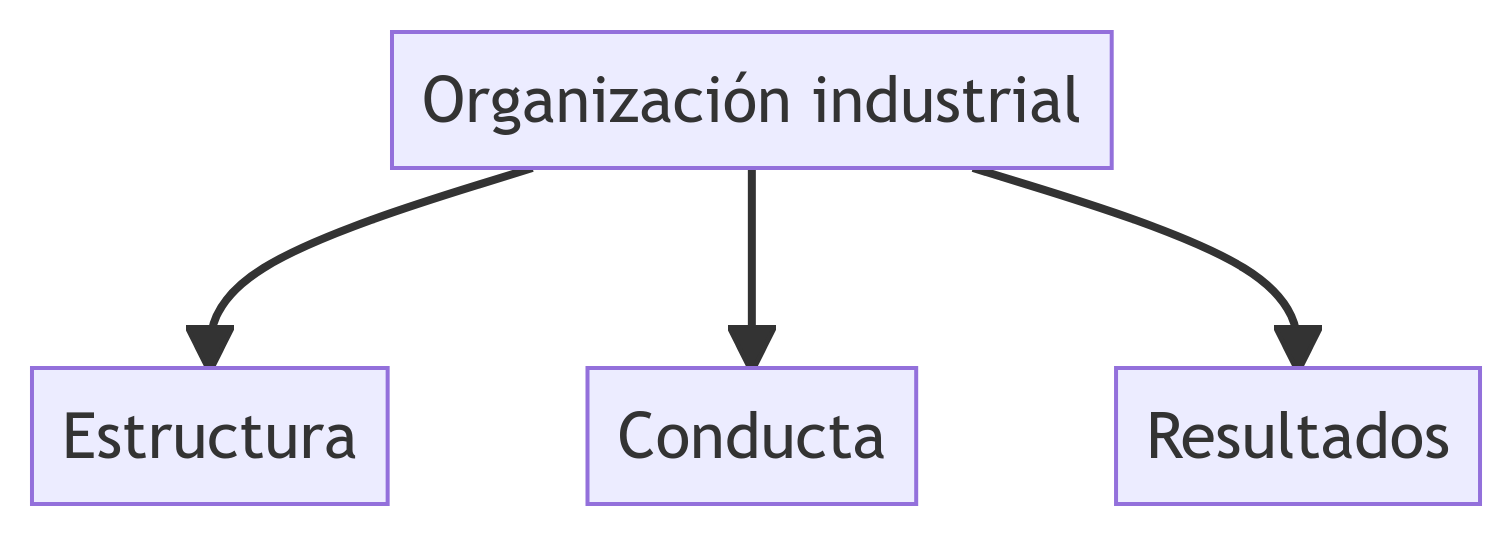
\includegraphics[width=3.94in,height=1.4in]{index_files/figure-latex/mermaid-figure-1.png}

}

\end{figure}

\hypertarget{estructura}{%
\subsection{Estructura}\label{estructura}}

Los elementos de la estructura en el análisis de la Organización
Industrial comprenden aspectos estáticos y dinámicos que influyen en el
funcionamiento de las empresas y el mercado. Algunos de estos elementos
son:

\begin{itemize}
\tightlist
\item
  Número y dimensión relativa de las empresas-clientes.
\item
  Diferenciación del producto.
\item
  Barreras de entrada y salida, incluyendo barreras naturales, legales y
  tecnológicas.
\item
  Estructura de costos.
\item
  Integración vertical, colusión, fusiones y cambios estructurales.
\end{itemize}

La estructura de la industria se puede representar mediante la ecuación
E = E(NEC, DQ, ESE, CFO), donde NEC representa el número y dimensión de
las empresas-clientes, DQ la diferenciación del producto, ESE las
barreras de entrada y salida, y CFO la estructura de costos.

\hypertarget{conducta}{%
\subsection{Conducta}\label{conducta}}

Los elementos de la conducta en el análisis de la Organización
Industrial se refieren a las prácticas y operaciones comerciales
llevadas a cabo por las empresas. Algunos de estos elementos son:

\begin{itemize}
\tightlist
\item
  Estrategias de precios, calidad y cantidad.
\item
  Estrategias de producto y publicidad.
\item
  Investigación y desarrollo.
\item
  Estrategias de inversión.
\item
  Grado de competencia.
\end{itemize}

La conducta de las empresas puede ser representada mediante la ecuación
C = C(O y D), donde O y D representan los elementos relacionados con las
estrategias y operaciones comerciales. Además, el poder y la
concentración también son factores que influyen en la conducta de las
empresas.

\hypertarget{resultados}{%
\subsection{Resultados}\label{resultados}}

Los elementos de los resultados en el análisis de la Organización
Industrial se centran en la eficiencia estática y dinámica de las
empresas y el mercado. Algunos de estos elementos son:

\begin{itemize}
\tightlist
\item
  Pleno empleo.
\item
  Distribución de los excedentes y beneficios económicos.
\item
  Eficiencia en la asignación de recursos.
\item
  Eficacia de la empresa, medida a través de ratios e índices de
  solvencia, liquidez o la Q de Tobin.
\end{itemize}

Los resultados obtenidos en el análisis de la Organización Industrial se
pueden representar mediante la ecuación R = R(DE; B, IS), donde DE
representa el pleno empleo, B la distribución de los excedentes y
beneficios económicos, e IS la eficiencia de los recursos.

\hypertarget{paradigmas-sobre-la-organizaciuxf3n-industrial}{%
\section{Paradigmas sobre la Organización
Industrial}\label{paradigmas-sobre-la-organizaciuxf3n-industrial}}

\hypertarget{el-enfoque-estructura-conducta---resultados}{%
\subsection{El enfoque: Estructura -- Conducta -
Resultados}\label{el-enfoque-estructura-conducta---resultados}}

El enfoque de Estructura-Conducta-Resultados (ECR) es fundamental para
comprender y analizar la organización industrial. Este enfoque sostiene
que cualquier estudio de la organización industrial debe considerar
estos tres aspectos de manera integrada, ya que son interdependientes y
proporcionan una visión completa de la dinámica del mercado.

\textbf{Estructura:} La estructura se refiere a la configuración de la
industria y abarca elementos como el número de empresas y clientes, la
diferenciación del producto, las barreras de entrada y la integración
vertical a través de colusiones y fusiones. Estos factores influyen en
la competitividad y el poder de mercado de las empresas.

\textbf{Conducta:} La conducta se relaciona con las estrategias y
acciones comerciales de las empresas. Incluye aspectos como los precios,
la publicidad, la investigación, la inversión en desarrollo e innovación
(I+D+i) y el grado de competencia. La conducta de las empresas determina
cómo compiten en el mercado y afecta directamente los resultados.

\textbf{Resultados:} Los resultados son las consecuencias de la
interacción entre la estructura y la conducta de las empresas. Incluyen
la distribución de los excedentes económicos, la rentabilidad, la
eficiencia en el uso de los recursos y la introducción de nuevos
productos o mejoras en la calidad. Estos resultados reflejan el
desempeño y la eficacia de la organización industrial.

Es decir, el enfoque ECR proporciona un marco analítico para comprender
la organización industrial en su conjunto, considerando la interrelación
entre estructura, conducta y resultados. Es esencial para evaluar el
poder y la concentración en el mercado y permite realizar estudios
complejos de manera simplificada mediante el uso de indicadores y
regresiones económicas.

\hypertarget{el-enfoque-de-eficiencia-ee}{%
\subsection{El enfoque de eficiencia:
(EE)}\label{el-enfoque-de-eficiencia-ee}}

El enfoque de eficiencia y eficacia (EE) se centra en lograr beneficios
tanto para la sociedad en general como para los productores
individuales. Este enfoque implica la utilización óptima de los recursos
disponibles, la maximización de la productividad y la minimización de
los costos. Además, considera la importancia de mantener un equilibrio
con el medio ambiente y promover prácticas sostenibles.

El mercado es el resultado de las interacciones entre los actores
económicos y está influenciado por aspectos normativos y de regulación.
El enfoque de eficiencia busca garantizar que las decisiones y acciones
de las empresas contribuyan al bienestar económico y social de manera
equitativa y sostenible.

\hypertarget{el-enfoque-del-crecimiento-con-investigaciuxf3n-desarrollo-e-innovaciuxf3n-idi}{%
\subsection{El enfoque del crecimiento con investigación, desarrollo e
innovación
(I+D+i)}\label{el-enfoque-del-crecimiento-con-investigaciuxf3n-desarrollo-e-innovaciuxf3n-idi}}

El enfoque del crecimiento con investigación, desarrollo e innovación
(I+D+i) destaca la importancia de invertir en actividades de
investigación y desarrollo para impulsar el crecimiento y la
competitividad de las empresas. Mediante la generación de nuevos
conocimientos, la mejora de productos y procesos, y la implementación de
innovaciones, las empresas pueden alcanzar ventajas competitivas y
adaptarse a los cambios en el entorno empresarial.

La inversión en I+D+i fomenta la creatividad, la generación de ideas y
la adopción de tecnologías avanzadas. Permite a las empresas
diferenciarse en el mercado, mejorar la calidad de sus productos y
servicios, y aumentar su eficiencia. Además, promueve la colaboración
entre diferentes actores, como empresas, instituciones de investigación
y organismos gubernamentales, para impulsar la innovación en la
organización industrial.

\hypertarget{el-enfoque-de-los-rendimientos-a-escala}{%
\subsection{El enfoque de los rendimientos a
escala}\label{el-enfoque-de-los-rendimientos-a-escala}}

El enfoque de los rendimientos a escala se refiere a cómo las empresas
gestionan su producción en relación con el tamaño de mercado y los
objetivos perseguidos. En este caso, las empresas pueden optar por
diferentes estrategias:

\begin{enumerate}
\def\labelenumi{\Alph{enumi})}
\item
  \textbf{Por el tamaño óptimo (CMeLP):} Las empresas pueden buscar el
  tamaño óptimo de producción que les permita minimizar los costos
  unitarios y maximizar la eficiencia. Esto puede implicar una
  estructura de costos constante (CMeLP constante), una estructura de
  costos creciente (CMeLP creciente) o una estructura de costos
  decreciente (CMeLP decreciente).
\item
  \textbf{Flexibilidad:} Algunas empresas optan por ser más flexibles en
  su capacidad de producción, lo que les permite adaptarse rápidamente a
  cambios en la demanda o en el entorno empresarial.
\item
  \textbf{Objetivos no económicos:} Algunas empresas pueden perseguir
  objetivos no exclusivamente económicos, como la tradición familiar, la
  creación y satisfacción de empleo propio, o objetivos sociales y
  políticos.
\item
  \textbf{Máxima producción según tamaño de mercado:} Las empresas
  pueden ajustar su producción para alcanzar la máxima capacidad de
  producción en relación con el tamaño del mercado en el que operan.
\end{enumerate}

Por lo tanto, el enfoque de los rendimientos a escala considera cómo las
empresas gestionan su producción en función del tamaño de mercado y los
objetivos perseguidos, teniendo en cuenta la eficiencia, la flexibilidad
y otros aspectos económicos y no económicos.

\hypertarget{la-economuxeda-positiva-y-la-economuxeda-normativa-en-la-organizaciuxf3n-industrial}{%
\section{La Economía Positiva y la Economía Normativa en la Organización
Industrial}\label{la-economuxeda-positiva-y-la-economuxeda-normativa-en-la-organizaciuxf3n-industrial}}

\hypertarget{economuxeda-positiva}{%
\subsection{Economía Positiva}\label{economuxeda-positiva}}

La \textbf{explicación} y \textbf{predicción} de fenómenos relacionados
con el funcionamiento de los mercados son los objetivos principales de
la economía positiva en el ámbito de la organización industrial. Se
busca comprender los precios y las cantidades de equilibrio en
diferentes estructuras de mercado, así como analizar la viabilidad de
prácticas comerciales como la colusión, la exclusión de competidores o
la discriminación de precios. También se examinan los cambios que pueden
ocurrir como resultado de fusiones o acuerdos horizontales o verticales
entre empresas.

\hypertarget{economuxeda-normativa}{%
\subsection{Economía Normativa}\label{economuxeda-normativa}}

En contraste, desde la perspectiva de la economía normativa, el enfoque
principal de la organización industrial es \textbf{evaluar políticas
públicas relacionadas con la intervención del Estado en el
funcionamiento de los mercados.} Se busca regular los monopolios y
promover la competencia como alternativas para abordar las distorsiones
generadas por el ejercicio del poder monopólico.

En este sentido, las distorsiones se resuelven a través de la acción
directa del regulador, quien toma decisiones en lugar de las empresas en
aspectos como precios, cantidad, calidad, inversiones, entre otros.


\printbibliography


\end{document}
